\documentclass[12p,a4paper]{article}
\usepackage[utf8]{inputenc}
\usepackage[T1]{fontenc,url}
\usepackage{multicol}
\usepackage{multirow}
\usepackage{parskip}
\usepackage{lmodern}
\usepackage{microtype}
\usepackage{verbatim}
\usepackage{amsmath, amssymb}
\usepackage{tikz}
\usepackage{physics}
\usepackage{mathtools}
\usepackage{algorithm}
\usepackage{algpseudocode}
\usepackage{listings}
\usepackage{enumerate}
\usepackage{graphicx}
\usepackage{float}
\usepackage{hyperref}
\usepackage{tabularx}
\usepackage{siunitx}
\usepackage{fancyvrb}
\usepackage[makeroom]{cancel}
\usepackage[margin=2.0cm]{geometry}
\renewcommand{\baselinestretch}{1}
\renewcommand{\exp}{e^}
\renewcommand{\b}{\boldsymbol}
\newcommand{\h}{\hat}
\newcommand{\m}{\mathbb}
\newcommand{\half}{\frac{1}{2}}
\renewcommand{\exp}{e^}
\renewcommand{\bar}{\overline}
\setlength\parindent{0pt}


\begin{document}
\title{MAT4110 -- Oblig 1}
\author{
    \begin{tabular}{r l}
        Jonas Gahr Sturtzel Lunde & (\texttt{jonassl})
    \end{tabular}}
% \date{}    % if commented out, the date is set to the current date

\maketitle

\hspace{10cm}

\section*{Exercise 1}
From lecture notes 4, we know that the least squared solution to the linear system
\[
    A\b x = \b b
\]
can be solved by QR factorization of A. We have that
\[
    ||A\b x - \b b||^2 = ||R\b x - Q_T\b b||^2    
\]
Further, let $R_1$ be the $m\times m$ upper triagonal half of $R$, and $\b c_1$ be the upper $m$ elements of $\b c$, where $\b c = Q^T\b b$.
The lecture notes show that the least squared problem is equivalent to
\[
    R_1\b x = \b c_1
\]
where $R_1$ is upper triagonal.

This has been implemented in Python, in the file QR.py, and run in the file oblig1.py. To avoid confusion with the x-axis named $\b x$, the coefficient vector is named $\b \beta$.

Below we see the results for the first dataset at the top, and the second below. m=3 is shown in the left, and m=8 on the right.
\begin{figure}[H]
    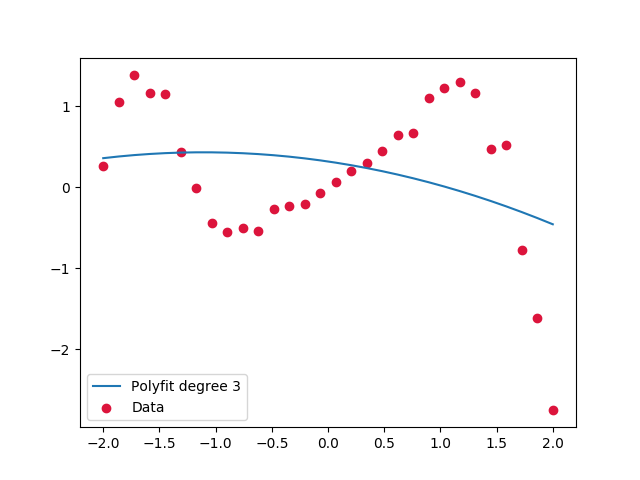
\includegraphics[width=0.5\linewidth]{../plots/QR_y0_m=3.png}
    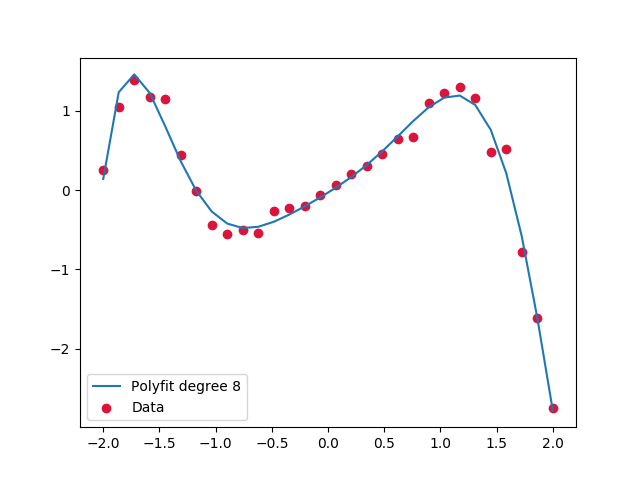
\includegraphics[width=0.5\linewidth]{../plots/QR_y0_m=8.png}
\end{figure}
\begin{figure}[H]
    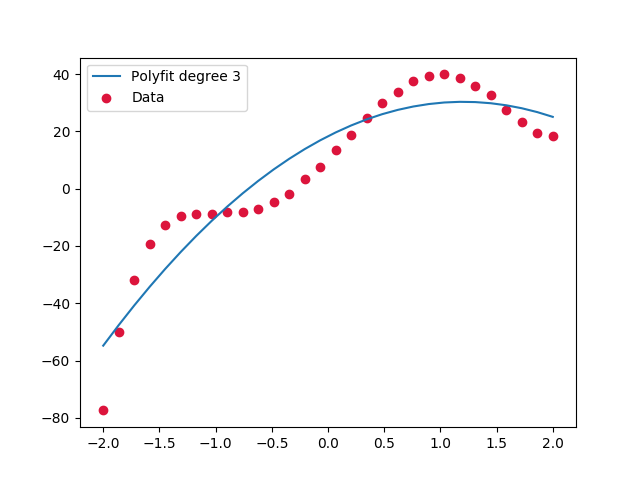
\includegraphics[width=0.5\linewidth]{../plots/QR_y1_m=3.png}
    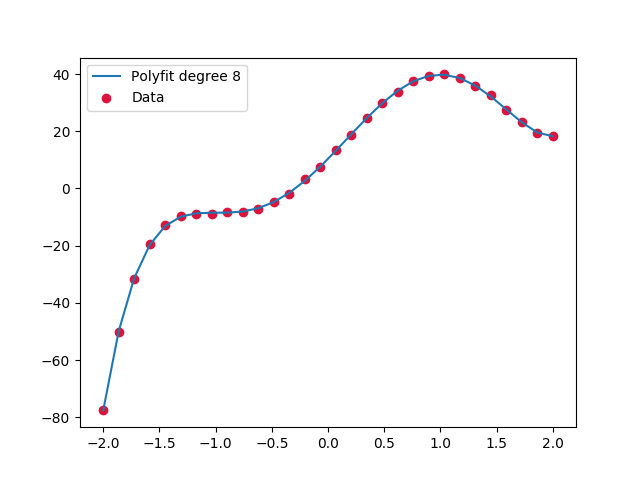
\includegraphics[width=0.5\linewidth]{../plots/QR_y1_m=8.png}
\end{figure}
    


\section*{Exercise 2}
The normal equation should solve the least squared problem for some $\b x$, and is given by
\[
    A^TA\b x = A^T\b b
\]
Recognizing that $B = A^TA$ is a symmetric, positive definite matrix, gives us the QR factorization $RR^T = B$. Inserting gives
\[
    RR^T\b x = A^T \b b
\]
$A^T$ and $\b b$ are known, and multiplying them gives
\[
    RR^T\b x = \b w
\]
where $\b w = A^T\b b$. This can be split into the two equations
\[
    R\b z = \b w
\]
and, having solved for z using backward substitution,
\[
    R^T\b x = \b z
\]
which can be solved using forward substitution.

This was implemented in Python, in the file Choleksy.py, and run in the oblig1.py file.

Below we see the results for the first dataset at the top, and the second below. m=3 is shown in the left, and m=8 on the right. They look identical to the ones we got from the QR factorization.
\begin{figure}[H]
    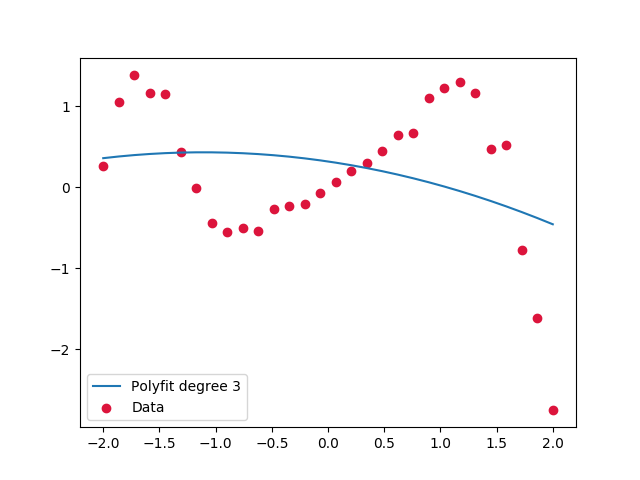
\includegraphics[width=0.49\linewidth]{../plots/cholesky_y0_m=3.png}
    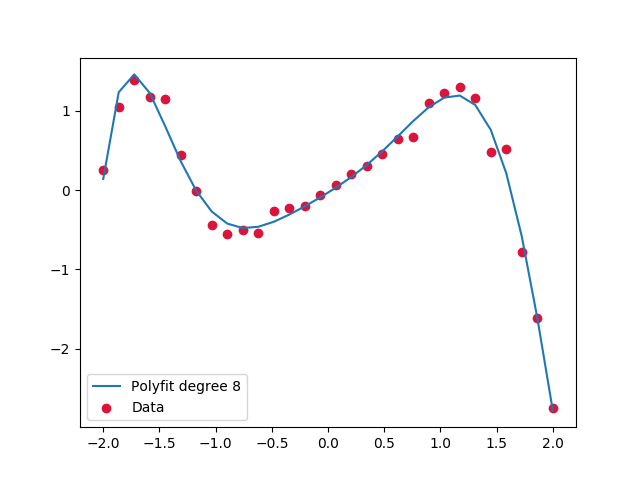
\includegraphics[width=0.49\linewidth]{../plots/cholesky_y0_m=8.png}
\end{figure}
\begin{figure}[H]
    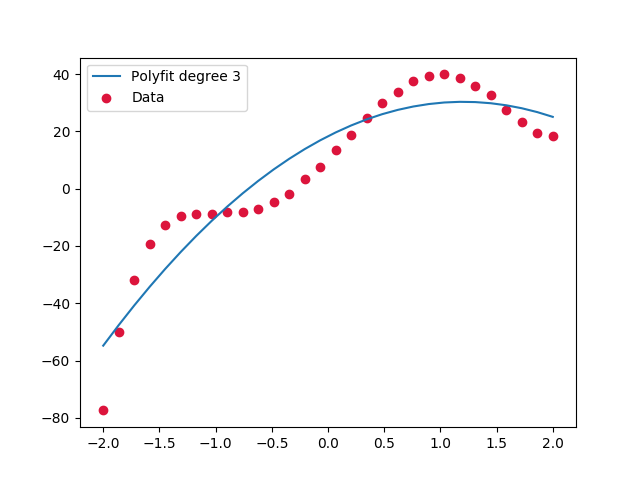
\includegraphics[width=0.49\linewidth]{../plots/cholesky_y1_m=3.png}
    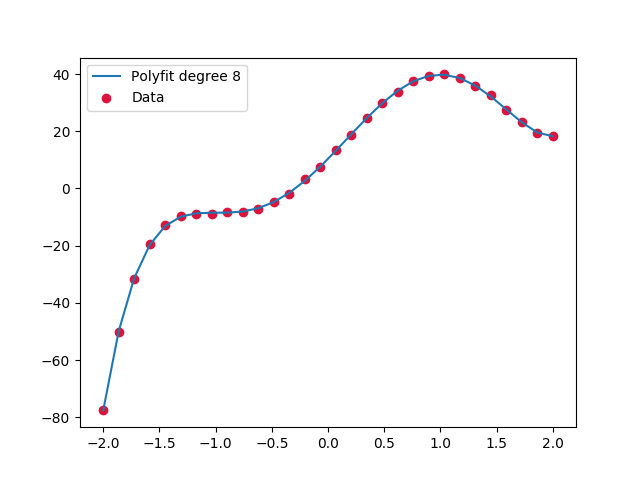
\includegraphics[width=0.49\linewidth]{../plots/cholesky_y1_m=8.png}
\end{figure}
    


\section*{Exercise 3}

Cholesky factorization involves taking the square root of quantities in $A$. This makes the algorithm especially sensitive to ill-conditioned matrices, as the square root has a very high loss of precision, compared to other operation.

I couldn't find any good sources on the behavior of QR on ill-conditioned matrices, but it uses Gram-Schmidt, which doesn't contain square roots, so I would imagine it plays more nicely.

The QR solver also seems to scale vastly better, in time, for larger polynomial degrees. Holding the number of points constant at $n=1000$, and increasing the polynomial order, we see from the plot below that Choleksy is much slower for large $m$, seemingly scaling as $m^{2.59}$ to QRs $m^{0.33}$ Granted, this doesn't look at the scaling with increased number of points.

\begin{figure}[H]
    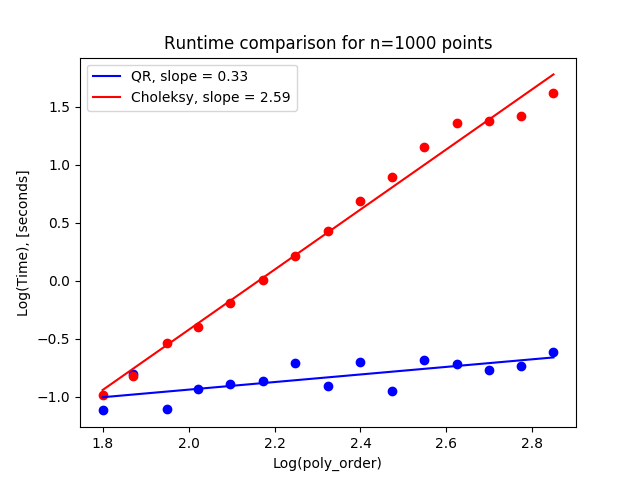
\includegraphics[width=0.80\linewidth]{../plots/timings.png}
\end{figure}


\section*{Appendix: Code}

\pagebreak

\lstinputlisting[language=Python, caption=oblig1.py, frame=full]{../src/oblig1.py}

\pagebreak

\lstinputlisting[language=Python, caption=QR.py, frame=full]{../src/QR.py}

\pagebreak

\lstinputlisting[language=Python, caption=cholesky.py, frame=full]{../src/cholesky.py}

\pagebreak

\lstinputlisting[language=Python, caption=tools.py, frame=full]{../src/tools.py}

\end{document}